\documentclass{article}
\usepackage{style}
\begin{document}
\maketitle
\tableofcontents
\section{Introducción}
Un historigrama es una representación gráfica de una variable en forma de barras, donde la superficie de cada barra es proporcional a la frecuencia de los valores representados. Con base en este definición se realizó un programa el cual grafica un historigrama con base en un arreglo de números aleatorios.
\section{Contenido}
\subsection{Ejemplo 1}
Ejecución: \textit{make \&\& ./historigram}
\begin{figure}[h!]
	\centering
	\caption{Ejemplo 1}
	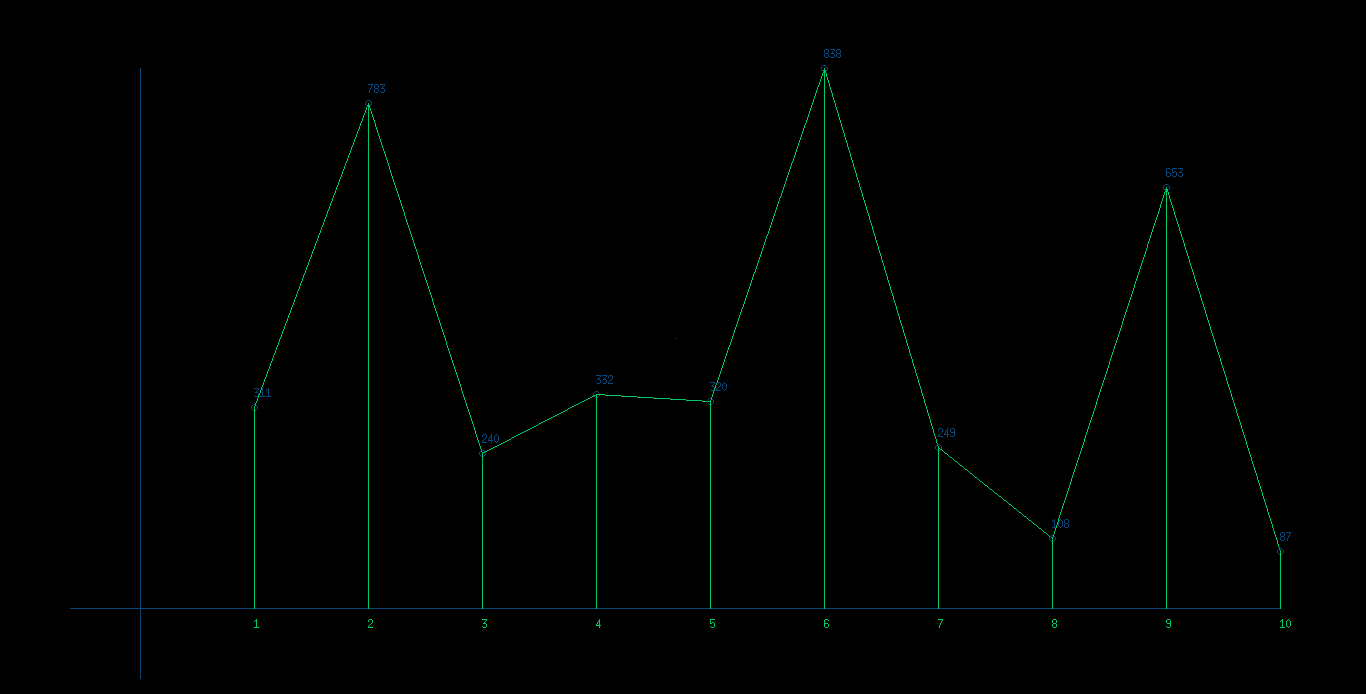
\includegraphics[scale=.35]{pantalla1}
\end{figure}
\newline
En este ejemplo se muestra el historigrama del arreglo: \textit{\{53, 56, 68, 54, 55, 15, 89, 81, 21, 36\}}\\
El programa por defecto crea un arreglo de 10 números aleatorios.
\subsection{Ejemplo 2}
Ejecución: \textit{make \&\& ./historigram 20}\\
\begin{figure}[h!]
	\centering
	\caption{Ejemplo 2}
	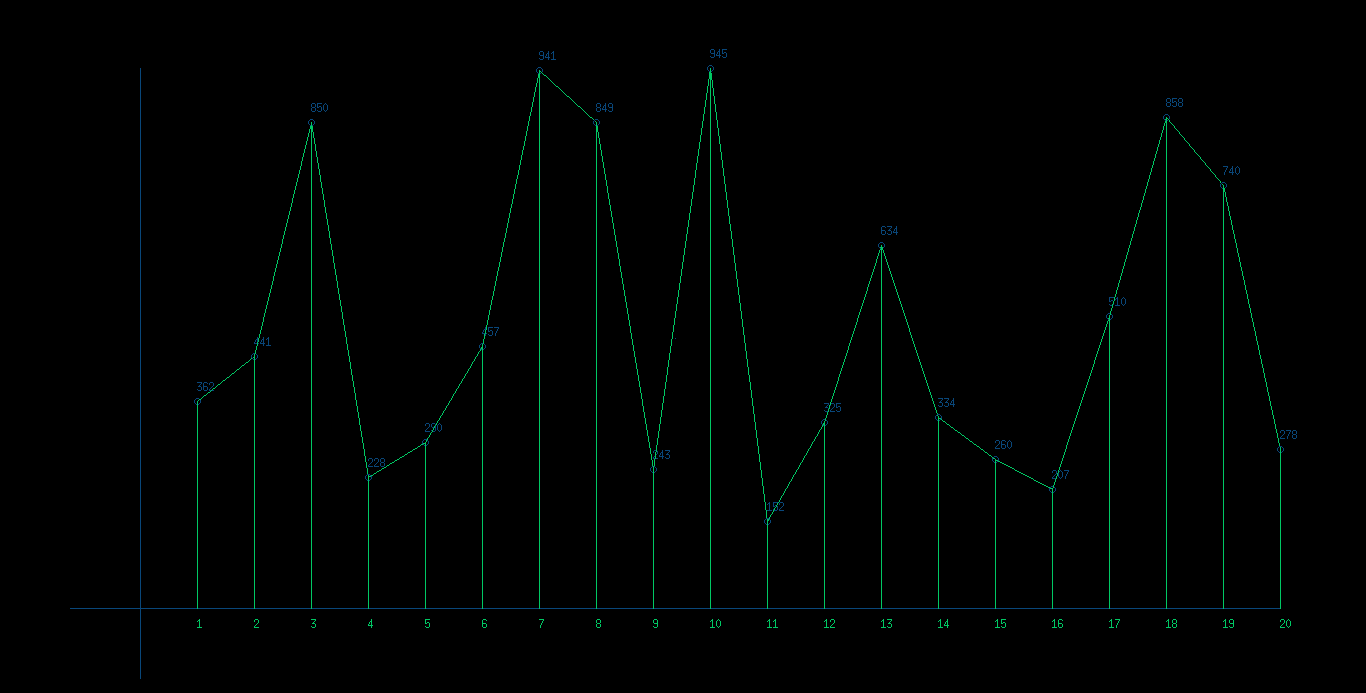
\includegraphics[scale=.35]{pantalla2}
\end{figure}
\newline
En este ejemplo se muestra el historigrama del arreglo: \textit{\{362, 441, 850, 228, 290, 457, 941, 849, 243, 945, 152, 325, 634, 334, 260, 207, 510, 858, 740, 278\}}\\
Se le dió un argument extra al programa que indica el número de elementos en el arreglo.\\\\
En ambos ejemplos los números aleatorios se generaron en nu rango del 1 al 1000.
\section{Conclusión}
Mediante un historigrama se pueden representar visualmente datos, lo cual hace que sea más fácil interpretar resultados y compartilos.
\end{document}